\section{Ergebnisse}
Das durch den Ferromagneten verursachte Magnetfeld ohne äußeres Einwirken wurde zu Beginn der Messungen auf $1.045(1) \unit{mT}$ bestimmt. Stellt man ein Magnetfeld von $190 \unit{mT}$ an Computer ein, misst das Teslameter $252.6(1) \unit{mT}$. Die Unsicherheiten sind hier in der letzten angezeigten Stelle des Teslameters. Am Ende der Messungen wurde das ungetriebene Magnetfeld gemessen um einen möglichen Drift (durch Magnetisierung des Eisens) festzustellen und es wurde ein Wert von $0.979(1) \unit{mT}$ gemessen. Dieser Effekt ist also vernachlässigbar klein. Der angelegte Strom von $I = 500 \unit{\micro A}$ wird während des gesamten Versuches nicht verändert und wird mit einem Fehler von $1.05\% \pm 0.5 \unit{\micro A} $ bestückt, welcher im Handbuch nachgelesen werden kann. Das sind genau $8 \unit{\micro A}$ und ist unter (späterer) genauerer Betrachtung der Fehlerkontributionen der dominierende Faktor.

Die aufgezeichneten Widerstands- sowie Spannungswerte wurden mit einer Unsicherheit von $0.05 \unit{\ohm}$ und $0.05 \unit{mV}$ respektive gewählt. Das Multimeter hat zwar eine Anzeige mit drei Nachkommastellen, die Werte verändern sich aber sehr schnell, was eine genauere Bestimmung durch händisches Ablesen und Aufschreiben sehr schwierig macht.

Zu Beginn werden die gemessenen Widerstandswerte mittels einer Kalibrierungskurve \autocite{hall} in Temperaturen umgerechnet (unter Berücksichtigung der Fehlerpropagation). Wir kommen bei normaler Zimmertemperatur nach Konversion in Temperaturen auf $T = 324.81(4) \unit{K}$, was etwa $25 \unit{K}$ über dem erwarteten Wert für Raumtemperatur liegt (es wurde leider keine Temperaturmessung mit einem anderen Messgerät durchgeführt, um die Richtigkeit der Kalibrierungskurve zu validieren). Da wir aber bei allen Widerstandsmessungen physikalisch sinnvolle Temperaturen erhalten (nichtnegativ, monoton fallend) wird mit einer potentiell fehlerhaften Kalibrierungskurve fortgefahren.

Folgend werden Widerstands- und Temperaturmessung synonymisch verwendet. Da die Temperaturmessungen immer nach vier Spannungsmessungen durchgeführt wurden, wurde über die Temperatur interpoliert. Um Messungen für den spezifischen Widerstand und den Hall-Koeffizienten später zu kombinieren, wurden die Temperaturen hier wieder gemittelt.

Um genauere Spannungsmessungen zu erhalten wurden immer zwei Messungen mit unterschiedlicher Stromrichtung durchgeführt und anschließend gemittelt.

Der Hall Koeffizient wurde mittels \autoref{eq:RH} bestimmt. Hier ist zu beachten, die Berechnung der Spannungsdifferenz richtig auszuführen, da sich hier leicht ein Vorzeichenfehler einschleichen kann. Der Hall-Koeffizient $R_{\text{H}}$ liegt bei \blockquote{Raumtemperatur} ($T = 324.81(4) \unit{K}$) bei
$$R_{\text{H}} = -0.0398(6) \unit{\cubic\m\per\C} .$$

$R_{\text{H}}$ hängt gemäß \autoref{eq:RHn} über der Elementarladung $e$ direkt mit der Ladungsträgerdichte $n$ zusammen, wobei das Vorzeichen vom Hall Koeffizienten die Art/Polarität dieser festlegt. Das negative Vorzeichen lässt auf n-Dotierung schließen, was einen Elektronenüberschuss impliziert mit Ladungsträgerdichte
$$ n = -\frac{1}{R_\mathrm{H}e} = 1.57(3) \cdot 10^{20} \unit{\per\cubic\meter} .$$

Den spezifischen Widerstand kann man über \autoref{eq:roh} bestimmen. Hier ist das Vorzeichen der Spannungen unwichtig, da diese im Betrag betrachtet werden (negatives $\rho$ ist unphysikalisch). Wir kommen bei Raumtemperatur auf
$$ \rho = 0.0802(13) \unit{\ohm\meter} . $$

Aus $R_H$ und $\rho$ lässt sich die Beweglichkeit der Ladungsträger $\mu$ über \autoref{eq:mu} bestimmen.
$$ \mu = 4961(13) \unit{\square\cm\per\s\per\V}. $$

Das Verhalten der freien Ladungsträger kann theoretisch modelliert werden \autocite{hall} und man erwartet sich ein konstantes Verhalten bei Raumtemperatur und einen exponentiellen Abfall bei niedrigen Temperaturen, wobei ein kontinuierlicher Übergang zwischen den beiden stattfindet. Um das exponentielle Verhalten sichtbarer zu machen, wurde die Ladungsträgerdiche $n$ logarithmiert, wobei zu beachten ist, dass $n$ in einheitenlose Form gebracht werden muss. In \autoref{fig:plot1} ist $\ln(n \cdot \oldunit{m^3})$ auf die inverse Temperatur $T^{-1}$ aufgetragen.

\begin{figure}[H]
    \centering
    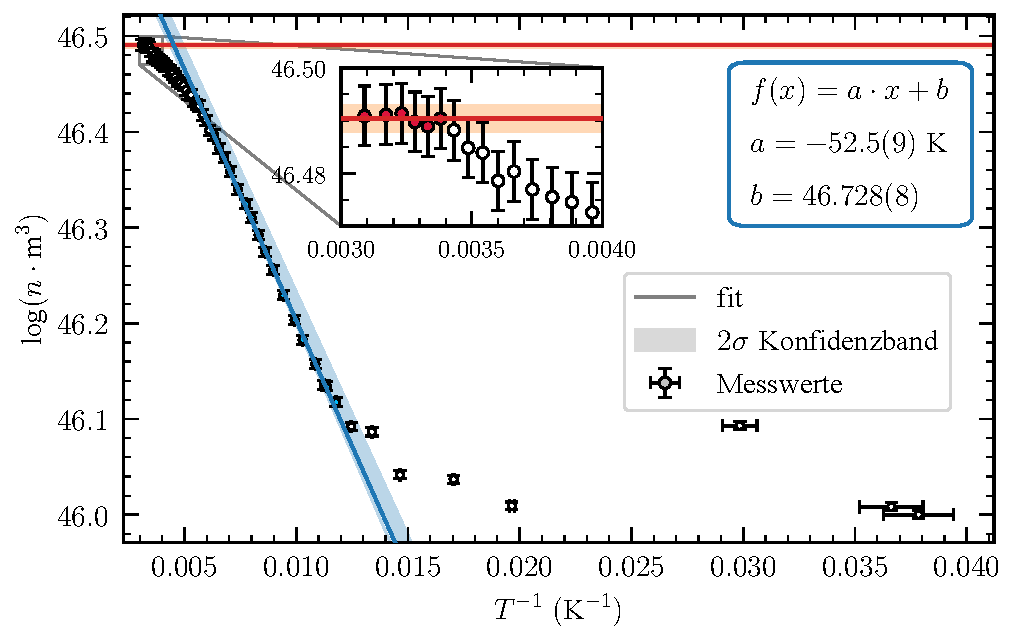
\includegraphics[width=\textwidth]{plot1.pdf}
    \caption{Der Logarithmus der bestimmten Ladungsträgerdichte $ n $ ist auf die inverse Temperatur $T^{-1}$ aufgetragen. Die Messpunkte sind mit $1\sigma$ Fehlerbalken in beiden Koordinaten ausgestattet. In orange wurde der gewichtete Mittelwert der ersten 6 Datenpunkten gebildet, wobei die dafür verwendeten Messwerte rot markiert sind. In blau wurde eine Gerade mittels ODR an die hellblau  gekennzeichneten Messwerte angepasst. Beide Geraden sind mit einem $2\sigma$ Konfidenzband bestückt.}
    \label{fig:plot1}
\end{figure}

Man erkennt das konstante Verhalten von $n$ bei Raumtemperatur (niedriger inverser Temperatur!) und das linear abfallende Verhalten vom Logarithmus sehr gut. Dazwischen befindet sich eine Übergangszone. Am unteren Ende der Temperatur weichen die Messwerte stark vom linearen Trend ab, da wir hier von dem PT100 Widerstand limitiert sind. Um den Ladungsträgerüberschuss zu messen, wurde aus Daten im konstanten Regime der Mittelwert gebildet. Dieser und die dafür verwendeten Messwerte sind in \autoref{fig:plot1} in orange zu sehen. Die Bandlücke $E_\mathrm{d}$ lässt sich mittels \autoref{eq:Ed} aus der Steigung der in blau angepassten Geraden berechnen. Die Geradenanpassung wurde über orthogonal distance regression (ODR) \autocite{odr} ausgeführt, um Fehler sowohl in x-, als auch in y-Richtung zu berücksichtigen. Wir erhalten folgende Werte für Ladungsträgerüberschuss und Bandlücke:
$$ N_\mathrm{D} - N_\mathrm{A} = 1.544(11) \cdot 10^{20} \unit{m^{-3}} \quad\text{und}\quad E_\mathrm{d} = 0.0091(4) \unit{eV} .$$

Aus $R_H$ und $\rho$ lässt nun sich die Beweglichkeit der Ladungsträger $\mu$ über \autoref{eq:mu} bestimmen. Diese ist in \autoref{fig:plot2} gegen die inverse Temperatur $T^{-1}$ geplottet.

\begin{figure}[H]
    \centering
    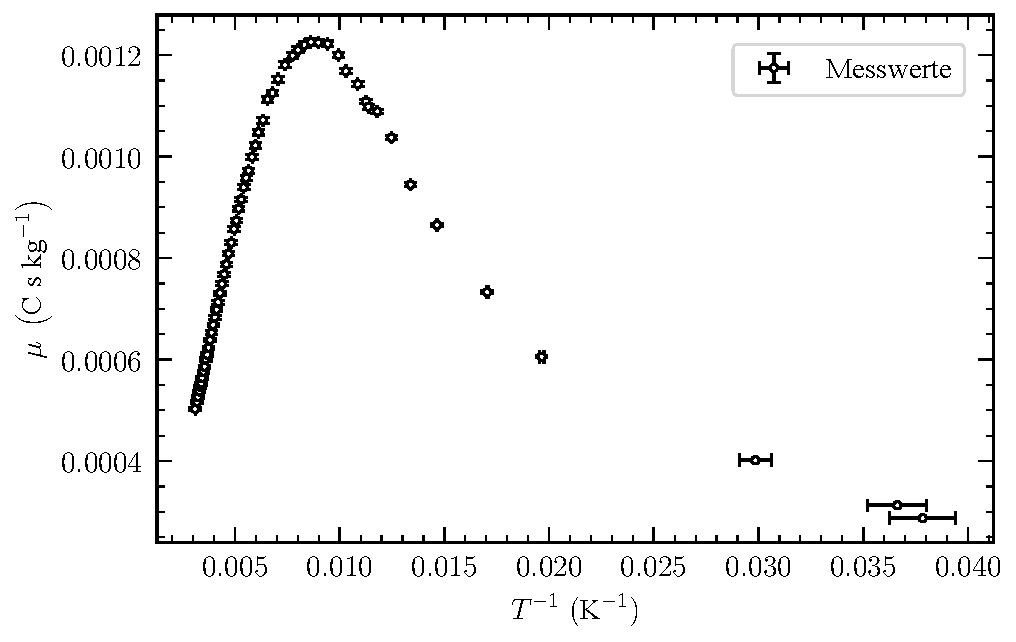
\includegraphics[width=\textwidth]{plot2.pdf}
    \caption{Die Beweglichkeit $\mu$ ist gegen die inverse Temperatur $T^{-1}$ aufgetragen. Die Messwerte sind mit $1\sigma$ Fehlerbalken bestückt, wobei diese bei hohen Temperaturen (und daher niedrigen inversen Temperaturwerten) sehr klein und in der Abbildung schlecht sichtbar sind.}
    \label{fig:plot2}
\end{figure}

Man erkennt in \autoref{fig:plot2}, dass $\mu$ mit abnehmender Temperatur ansteigt, ein Maximum bei etwa $110 \unit{K}$ erreicht und danach wieder absinkt. Aus der Theorie wissen wir (siehe \autoref{sec:Streuung}), dass verschiedene Mechanismen in einem Festkörper für die Veränderung der Beweglichkeit verantwortlich sind, die bei unterschiedlichen Temperaturen stattfinden. Diese hängen mit unterschiedlichen Potenzen von der Temperatur ab, weshalb ein doppellogarithmischer Plot der Beweglichkeit $\mu$ gegen die Temperatur $T$ in \autoref{fig:plot3} zu sehen ist.

\begin{figure}[H]
    \centering
    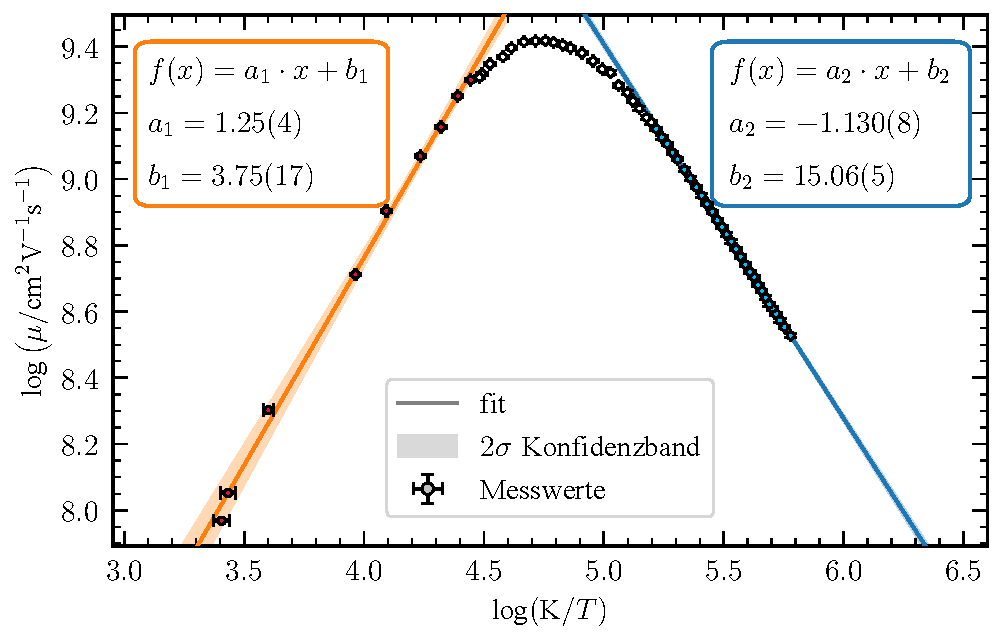
\includegraphics[width=\textwidth]{plot3.pdf}
    \caption{Der Logarithmus der Beweglichkeit $\mu$ ist auf den Logarithmus der Temperatur $T$ aufgetragen. In orange (blau) wurde eine Gerade an die Daten bei niedrigen (hohen) Temperaturen angepasst, die für die beiden Fits verwendeten Daten sind hier farblich markiert. Beide Geraden sind von $2\sigma$ Konfidenzbändern umgeben.}
    \label{fig:plot3}
\end{figure}

In \autoref{fig:plot3} sollten reine Potenzabhängigkeiten als Geraden mit der jeweiligen Potenz als Steigung erscheinen. Da zwei Streumechanismen erwartet werden, wurden zwei Geraden an die Daten angepasst, eine bei niedrigen Temperaturen (orange) und eine an Hohe (blau). Die Fits wurden wieder mit ODR durchgeführt und die für die Fitroutine verwendeten Daten wurden optisch passend gewählt und farblich markiert. Die Steigungen der beiden Geraden sind
$$ a_1 = 1.25(4) \quad\text{und}\quad a_2 = -1.130(8),$$

wobei $a_1$ die phononische und $a_2$ Rutherfordstreuung charakterisiert.
